\chapter{Bay-Delta SELFE Application}
\section{Application introduction}
Thus far we have described the SELFE model in the sense that it is an algorithm or piece of software,
including modifications (hydraulic structures and mass sources) that we made as part of the current project.
In this section we describe the {\em model application}; viz, the model configuration including 
the extent of the domain, mesh, initial and boundary conditions needed to drive the model. 

\section{Datum and units}
For spatial data, the project projection is NAD 1983 UTM Zone 10N based on North American Datum 1983.
The vertical datum is NAVD88 (North American Vertical Datum 1988), and this is the datum used in the 
model to partition total depth into unperturbed bathymetric depth and free surface elevation (see 
Figure \ref{fig:depths}).

The model calibration is configured in SI units, which are assumed in SELFE. Results are also 
given in SI units but English units are indicated on many of the plots.

The unit of salinity used inside SELFE is the \gls{psu} as defined by the 
Practical Salinity Scale of 1978 (PSS-78). While standard in oceanography, 
the PSU is sometimes an unfamiliar unit to Delta modelers and managers. 
It is virtually identical to parts per thousand (ppt) of salt -- 
a somewhat more familiar unit used to define some of the Delta water quality standards.
For instance, X2 happens where bottom salinity is 2 psu.

The more common way of observing salinity in the Delta is through the surrogate \gls{ec}.
In fact, when agencies (USGS and NOAA) report salinity in PSU (rather than ionic concentrations
such as chlorides), the practical salinity is back-calculated from EC.
Given the importance and familiarity of conductivity, in this document we
 often include conductivity in plots on a second axis. 
Conductivity is give in $\mu$Siemens/cm at $25\,^{\circ}\mathrm{C}$, which 
is an SI unit equivalent to $\mu$mmhos/cm. The (nonlinear) relationship between EC and
salinity is the one quoted by \cite{suits2002} including the Hill correction in the dilute range 
below 2.0 psu but not including corrections for agricultural salt. This relationship is shown in
Figure \ref{fig:ec_psu}, which also demonstrates the smallness of the Hill correction.   

\begin{figure}
	\centering
		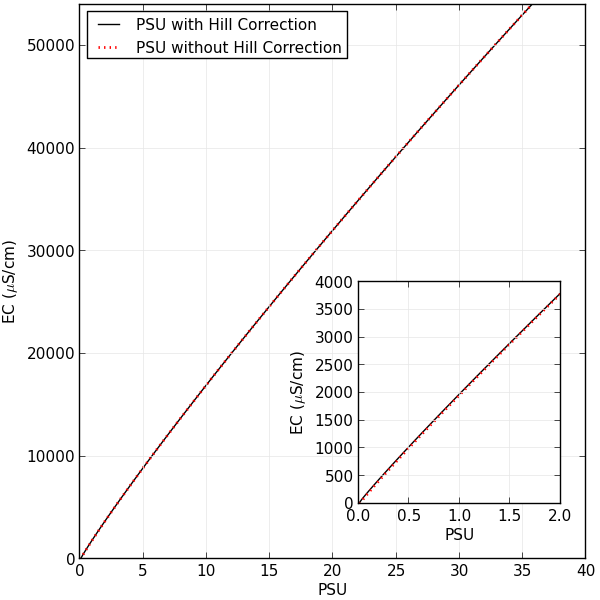
\includegraphics[scale=1]{image/ec_psu}
	\caption{Relationship between Practical Salinity Units (psu) and Conductivity 
	  ($\mu$S/cm at $25\,^{\circ}\mathrm{C}$) for the full range (main plot) and low (inset) salinity.}
	\label{fig:ec_psu}
\end{figure}

\section{Mesh}
\label{sec-delta-mesh}
The full Bay-Delta mesh is shown in figure *** and four example sections of the horizontal mesh are shown in Figure***. 
The mesh presented in this calibration comprises ~210000 triangles and ~130000 nodes. 

The Bay-Delta Mesh was constructed using the Aquaveo SMS generic software package, in which the user first specifies a 
skeleton {\em mesh map} comprised of discretized polygons (which can come from contours, 
GIS polyline coverages or simply be hand-drawn), each of which is then filled using 
one of several automatic meshing algorithms. Local resolution is controlled by
the spacing between vertices in the line segments of the mesh map as well as control points. Dense maps representing 
mesh size functions can also be provided by the user, but this option was not utilized in the present project.

Two generation algorithms are employed. An advancing front algorithm ("paving", figure **) is used for 
larger, well-resolved regions and also in some side embayments. Advancing front methods work particularly well in areas
like the coastal part of the model where the body of the polygon to be filled is large in every dimension compared
to the discretization length. Coons patches ("patching", figure **) are used in channelized areas, including the main part of Delta channels and the internal channels in some bays and open water bodies. The advancing front method produces more optimally shaped (ie, equilateral) triangles but is difficult to control in tight areas so that it conforms to bathymetry well. The
Coons patch looks more like a curvilinear grid and can follow and resolve sinuous channels or contours. Figure *** compares
the result of a Coons patch with paving for a narrow channel.

The SELFE Bay-Delta mesh resolution varies from approximately 1km in the ocean, 100-400m in the Bay and down to 15-60m in Delta
channels, with the smalles element size of ~2.5m found near some narrow channels of Middle River. The mesh sizing was chosen
\begin{itemize}
	\item to resolve bathymetric features and the deep sections of major channels (including internal channels in bays)
	\item to resolve lateral and vertical variation in velocity, as determined by sensitivity studies on velocity and
	salinity transport
	\item to emphasize regions of policy importance or that have a greater effect on global accuracy
	\item to take good advantage of SELFE's ability to handle anisotropy and non-orthogonality robustly in less resolved areas (our
experience suggests that the model can effectively handle skew elements with skewness up to 20).
	\item to realistically introduce wetting and drying while keeping always-wet main channels open to flow
	\item with consideration given to time step (CFL) implications, emphasizing regions that could be refined without introducing 
	excessive numerical diffusion (in ELM) or subcycling and performance issues (transport, particularly with the TVD algorithm).
\end{itemize}

These criteria were supported by numerous prototype meshes and informal sensitivity studies, 
particularly in the Carquinez Strait and Suisun Marsh. Although we are aware of automata 
that may support many of these criteria (most notably \cite{Persson2004,Persson05}, and
on simple reaches these methods produce very beautiful meshes. However the resulting loss functions
for mesh size are complex and implementing them will require specialty additions to software. 
In contrast, most general purpose meshing software is overly dedicated to either 1) measures of local accuracy
or 2) boundary curvature (ie, the shores, not the contours that delineate the deep part of the channel).
 
Modeling narrow channels and openings efficiently requires some care with SELFE, because the free surface (stage)
is modeled at mesh nodes and care must be taken that the wetting and drying rules 
(see Section \ref{subsec-wet-dry-grid}) do not engage prematurely and choke off the channel at low tide. This is not much of a restriction in larger, well-resolved channels such as the Sacramento *** (figure ***) where less than *** of the channel area
and most of the bathymetric uncertainty is concentrated on the levee slope (see \citet{Wang12}). For narrower channels
that are not resolved 5-6 elements across such as the Mokelumne, the meshing strategy shown in Figure *** is used whereby the levee slope is either ignored (left bank) or nodes are carefully placed to resolve the bank (right).


The overall shallowness of the Bay-Delta system allows us to use the terrain-following coordinate system ($S$) alone without $Z$
layers, thus avoiding a staircase grid everywhere. We set a modest value for the stretching constant ($\theta_f=1$) and chose ($\theta_b=0.5$) so more resolution is placed near the surface  than near the bottom. The transition depth at which $S$
reverts back to traditional $\sigma$ coordinate system was set at $h_c=10m$, and so only the deeper channels are discretized using
$S$, whereas vast shallow areas use $\sigma$. After some sensitivity tests, the total number of levels was fixed at 23.

One outside commentator were curious why we did not use hybrid coordinates to avoid over-resolving the upper estuary. 
The issue can be seen in Figure \ref{fig:vgrid}. The number of S levels has to be set to 
adequately revolve the deepest water. In our case, this is the 
Golden Gate at 100m and the resulting number of layers is 23. This is clearly more 
than necessary in the channels upstream which might be 4-10m deep. Although this represents
a potential inefficiency, experience by SELFE users on other basins apparently indicates two reasons not to use
SZ hybrid grids unless absolutely necessary: reduced accurate from the stairstepping Z grid and
a potential small numerical boundary layer caused by the transition from S to Z. We are currently 
developing a mesh based on pseudo-sigma coordinates similar to those used by \citet{Dukhovskoy09} but without the
stairstep noted by \cite{Siddorn13}. A pseudo-sigma coordinate system is terrain-following like an S-grid
but allows S levels to vanish in shallower water. The primary advantage to pseudo-sigma coordinates, as with SZ,
is to flatten the levels in steep topography and improve pressure calculations. However, it can be configured in
a way that that has the ancillary benefit of reducing vertical resolution in upstream areas.


\section{Bathymetry} 
SELFE requires bathymetry data at every node in the mesh. Bathymetry preparation for multidimensional modeling is described in \cite{Wang12}. 

Our bathymetry integrates elevation data from previous USGS maps, single and multibeam data collections into a set of consistent 10m and 2m elevation DEMs. 
The data used in calibration is identical to the Version 2 release of this bathymetry except that here 
we have incorporated recent improvements near the CVP intake and South Delta, 
and some additions in the North Sacramento where we extended the bathymetry in response to boundary reflection. Artificial deepening was performed at a small number of nodes 
(fewer than 0.1\%) to reinforce the connectivity or conveyance of the channels in areas where photography indicates error in the 
DEM or where underresolved shallow undulations were detrimental to model performance.




\subsection{Volumetric and face optimization}

Once the mesh is fixed, the bathymetry is assigned to the nodes of the model
 in such a way as to ensure fidelity not only to the point value 
of the bathymetry at nodes (which are where SELFE stores  bathymetry) 
but also to the volume of the elements and to the area of the 2D vertical faces 
along the edges of the mesh. 

This volume and area matching is performed by solving a weighted, regularized 
least squares problem that penalizes differences between the SELFE representation of the bathymetry
(which amount to a TIN) and the result of much denser Gaussian integration over the elements and sides.
All samples from the DEMs are taken using bilinear interpolation from the best quality DEM available for the 
requested point.

\begin{align}
   &\Min_{z_n, n=1,N_p}
   \begin{aligned}[t]
      &\sum_{e=1}^{N_e} \frac{1}{A_e}(V_e - V_e^q)^2 + \beta_s \sum_{s=1}^{N_s} \frac{1}{l_s}(A_s-A_s^q)^2 \\
      & + \alpha_n \sum_{n=1}^{N_p} (z_n-z_n^{0})^2 + \alpha_s \sum_{s \in \Gamma_{l}} (\Delta z)_s^2
   \end{aligned} \notag \\
\end{align}

where:
\begin{align*}
&N_e, N_s, N_p  &\text{number of elements, sides, nodes} &\\
&\Gamma_{l}  &\text{set of all sides on land boundaries} &\\
&V_e            &\text{volume of element (SELFE)} &\\
&V_e^q          &\text{volume of element (quadrature)} &\\
&A_e            &\text{horizontal area of element (SELFE)} &\\
&A_s            &\text{vertical area of side (SELFE)} &\\
&A_s^q          &\text{vertical area of side (quadrature)} &\\
&l_s            &\text{length of side} &\\
&z_n            &\text{elevation assignment} &\\
&z_{n}^{0}    &\text{original elevation from DEM } &\\
&\Delta z_n     &\text{(undivided) difference in elevation along side}  &\\
&\beta_s        &\text{weight of area}  &\\
&\alpha_n, \alpha_s  &\text{regularization weights} \\&
\end{align*}

The first two terms of the loss function penalize deviations in volume and area. The last two are
small Tikhonov-like regularization terms that penalize deviations from
the original point values interpolated from the DEM and also penalizing sharp fluctuations 
along land boundaries. The loss function weighs elements equally so it is 
not quite the discretization of a continuous problem.

The result of this optimization process is a small vertical adjustment to the depth assignments at nodes, which is where SELFE
stores bathymetry. Figure \ref{fig:optimization} gives some indications to what extent optimization can make up for volumetric error. The difference in element-averaged bed depth (based on a reference surface of ***) 
is shown for the SELFE representation shape functions and 14-point quadrature. 
Four cases are shown -- two different meshes, each with and without quadrature. 
Mesh 57 was a manual reworking of mesh 50,  specifically aimed at delineating the foot and top of slopes along the Sacramento.  
The figure clearly shows that the optimization can reduce error but the improvement is not a substitute for good horizontal placement of the nodes.
 
\begin{figure}
	\centering
		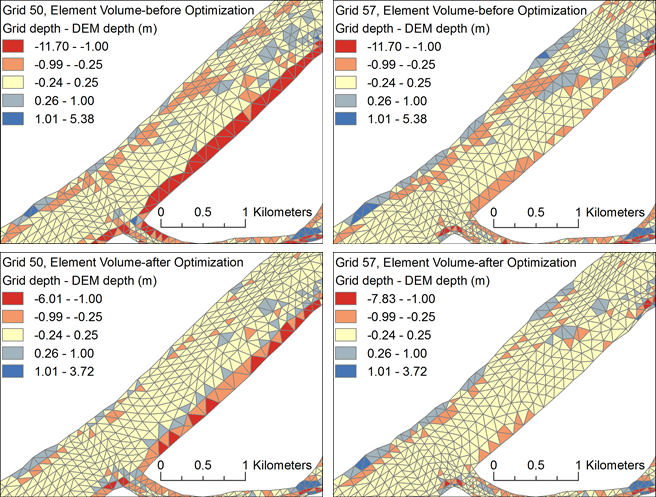
\includegraphics[scale=1.00]{image/optimization}
	\caption{Volume discrepancies for two versions of the mesh, before (top) and after (bottom) volumetric optimization.}
	\label{fig:optimization}
\end{figure}


We have verified that this bathymetry cleanup produces better flows at most sites. 
One unanticipated benefit of the optimization is the suppression of
 unrealistic undulations on the shore prevents erratic wetting and drying. The difference in the shoreline is shown 
in Figure ***, which compares a shore segment before and after optimization. 

The optimization does relinquish 
some of the control over elevations that can come from, say, very close digitizing along contours. 
This control can be an issue when planning for adaptive aspects of the algorithm that 
depend on depth thresholds, such as the switching between TVD and upwind transport schemes. In such cases, 
one usually wants to mesh just above or below the TVD threshold. 




\subsection{Deepening near boundaries}
SELFE does not restrict the value of inflows in any way (zero or withdrawal is fine), but it does not allow boundaries to become
dry. This modeling requirement is not at odds with our desire to extend the mesh up the major rivers beyond the region of tidal influence, but
it does raise some practical problems with initial conditions and boundary conditions at startup. If we na\"{\i}vely
initialize using a water surface gradient based on interpolation or steady state principles, the initial transient can 
behave like a flood wave. What we have found is easier is to use a flat water surface at a reasonable high tide value and impose
a maximum bed elevation near the boundary that will be wet at this level (Figure ***). Our experiments indicate no appreciable
sensitivity to this treatment.


\section{Initial conditions}
SELFE requires an initial condition for the entire model state, including velocity, water levels and salinity. Because the main
tidal hydrodynamic information propagates very quickly from the boundaries to the rest of the system, the domain has only a brief
memory (2-3 tide cycles) of velocity and surface elevation initial conditions. As long as the salinity field is reasonable (to
stabilize baroclinic movements), the main criteria in selecting elevation and velocity initial conditions are practical ones: to
minimize startup transients and maximize compatibility with boundary conditions. These goals are easier to achieve with very simple
flow fields; hence we cold start these variables from a velocity of zero everywhere and an elevation of 0.96m NAVD 
which is a medium-high tidal water level. To increase compatibility between the velocity and boundary conditions (which, when careless introduced into a non-diffusive model often result in mini-tsunamis or water hammers), the elevation and velocity
boundary conditions are ramped up linearly from zero over a few days. 

The system memory for salinity is much longer -- at least several months -- and it is helpful if the salinity initial condition roughly captures field conditions particularly in the Bay. The salinity initial condition was generated regionally:
\begin{itemize}
	\item Ocean: A scalar value of 33.5 psu at all depths,  which is typical of the shelf region at modest depth \citep{Dever94}.
	\item Bay and Suisun: From the South Bay to the confluence the model is initialized using \gls{ctd} casts from USGS water quality cruises, interpolating linearly longitudinally between stations and extrapolating radially as a constant from the centerline of the cruise.
	\item Delta: A scalar constant value of 0.1 psu (213 $\mu$S/cm EC) throughout the Delta. This value is typical for the north Delta but probably relatively fresh for the South Delta.
\end{itemize}

To minimize the influence of salinity initial conditions from our March 12, 2009 calibration simulation start date, we do not generate salinity skill statistics before June 1, 2009 for the Delta and May 1, 2009 for the Bay.

Some ongoing effort is underway to minimize spinup time by briefly (March 12-15 in this case) assimilating data from observation stations in the Delta through nudging (Newtonian Relaxation). SELFE has the ability to assimilate data in this manner, but time did not allow us to complete the data preparation work in time for this document. 

\section{Ocean boundary}
  \label{ocean-boundary}

\subsection{Boundary placement}
In order to use our model for processes that extend to the ocean (salt intrusion under sea level rise, full life cycle salmon modeling) the boundary of the model must be far enough offshore so that the dynamics of the domain do not impact the boundary. The ocean boundary of the Bay-SELFE model lies on a roughly 46km radius arc from the Golden Gate, extending from Point Reyes to the Farallon Islands and south just past Half Moon Bay (Figure ***). This shape and placement is similar to the boundary described by \citet{Chua2011} in their  model of the San Francisco Bay using SUNTANS. An alternative is described by \citet{MacWilliams08,MacWilliams09} in their UnTRIM application; they use a straight boundary oriented along isobaths in the alongshore direction.
%
Our placement of the boundary attempts to reconcile these conflicting factors:
\begin{itemize}
\item The size of the likely temperature, fresh water or sediment plume.
\item The orientation of bathymetry and likely propagation directions of tidal constituents
\item Structure of currents
\item The model coupling to ROMS in the SESAME project
\item Locations of available boundary tidal information.
\end{itemize}

The primary consideration was containing the freshwater jet and plume from the Bay on ebb tide, which we felt was easier to do with the semi-circular boundary configuration. Figure \ref{fig:plume2} shows a snap shot of the sediment plume exiting from the San Francisco Bay (**permission). \citet{Hurst08} have described evidence of plume fronts as far as 122.66\textdegree W (indicated***), or roughly 20km from the Golden Gate.
\citet{Carlson74} analyzed aerial photos of sediment plumes in the early 1970s and observed plumes approximately 30km from the Golden Gate during high outflow periods in 1970 and 8km during lower, more typical, outflow conditions. Using satellite imagery supported by in situ measurements, \cite{Ruhl01} measured sediment plumes at 15km from the Golden Gate based on suspended sediment, although the pertinent figures in that paper suggest that above-ambient sediment concentrations farther (perhaps 30km). 

At 45-46km from the Golden Gate, our domain should contain the fresh water plume under all but the most exceptional conditions. This
distance is also a maximum practical size of the domain. [b.c. is the main concer as you pointed out] 
 Locating the ocean boundary entirely on the shelf is preferable to partially extending it to the continental slope.
This is particularly the case off the California coast -- the summary by \citet{Noble2001} indicates a significantly
different tide and current pattern on the shelf and slope. Nuanced differences such as these would not be reproducible without data assimilation, very detailed boundary conditions and improved atmospheric data, none of which is possible to provide in a hypothetical planning context 
and which are unlikely to improve global accuracy in areas of greatest policy interest in the interior Delta.

Although we selected the arc as our boundary, the orientation of the bathymetry and tidal propagation suggests some important
hydrodynamic features vary most simply along the straighter isobaths that run in the alongshore direction of the greater Califonia
coastline. Figure *** shows contours of local bathymetry and makes this direction clear; Figure *** shows predicted isocontours of
amplitude and phase of the largest semi-diurnal (M2) and diurnal (K1) tidal constituents along the near coast according to WEBTIDE,
 a modeling product that uses data assimilation and ocean dynamics to map tidal constituents. Inasmuch as a trend is evident, it follows the alongshore direction. We had some difficulty validating these spatial trends of constituents in field data, in part because of the local character of some of the records such as Bolinas Bay. 

The orientation of currents is much less predictable. Large scale trends in mean currents tend to vary depending on season and whether upwelling is occuring.  Patterns observed using tidally averaged 6km HF Radar (***) also indicate a number of local current patterns offshore forced by prevailing winds and bathymetry such as the promontory of the Point Reyes peninsula. Given the small magnitude and peculiarities of velocities offshore and our inability to reproduce them in a planning setting, we use the alongshore variation in tidal constituents in preparing our surface boundary data, not in the orientation of the boundary or prescription of velocity. 

\subsection{Boundary data}
When used in 3D hydrostatic mode which is the typical mode of calculation of all the regional 3D models when applied on the full Bay-Delta domain, there is some freedom -- or ambiguity -- in the number of boundary conditions required on the ocean boundary. As a practical matter this ambiguity rests on whether velocity is needed -- tidal water levels are always supplied. 

For water levels, our model uses an inverse-distance combination of two stations, one at Point Reyes and one at Monterey. 
These are prefiltered using a low-pass filter with a cutoff frequency of 1 cycle/hr
 to remove obvious high frequency oscillations and then disaggregated around the boundary using
inverse-distance interpolation. We found this gave better water surface results in the interior domain in our model than the single station methods based on a lagged San Francisco tide \citep{MacWilliams08,MacWilliams09} or Point Reyes \citep{Chua2011}, and it also induces a small flow across the ocean segment of the domain that we hope sweeps the plume away at a rate that is representative of at least the tidal component of alongshore current. The boundary conditions are easy to synthesize in planning scenarios using an astronomical forecast with or without long period wave adjustments or storm surge.

The model can run on water levels and salinity alone (in 2D this would be routine). However, we feel the boundary is underspecified in 3D (the reason we use subjective language here is the general ill-posedness of the 3D shallow water hydrostatic equations near open boundaries \citep{Oliger78}.
As a result, we also prescribe the full velocity field along the (3D) boundary, but that velocity is synthetic. To generate the
synthetic velocities, we use the barotropic-baroclinic sequence described in section ***. In a separate effort, we are also
collaborating with a ROMS team to use their model velocity results as our b.c.

\begin{itemize}
	\item A preliminary 2D (or, occasionally 3D) barotropic run using diffusive numerical settings to generate simple velocities along the boundary and
	\item A 3D hydrostatic, baroclinic run using the barotropic velocities as boundary conditions.
\end{itemize}

Although this leads to some extra effort and workflow complication, the 2D barotropic run is extremely fast compared to the 3D baroclinic run so there is little increase in runtime. The resulting velocities are better behaved near the boundary -- our experience using 32 vertical layers was that underspecifying the boundary by using only tidal water levels led to unplausible high velocity fluctuations at the boundary, particularly along the ****canyon (Figure ***). There is no 'correct' treatment of this issue, as it arises from the hydrostatic equations.  
The rest of the domain is very insensitive to the boundary velocities. 

\begin{figure}
	\centering
		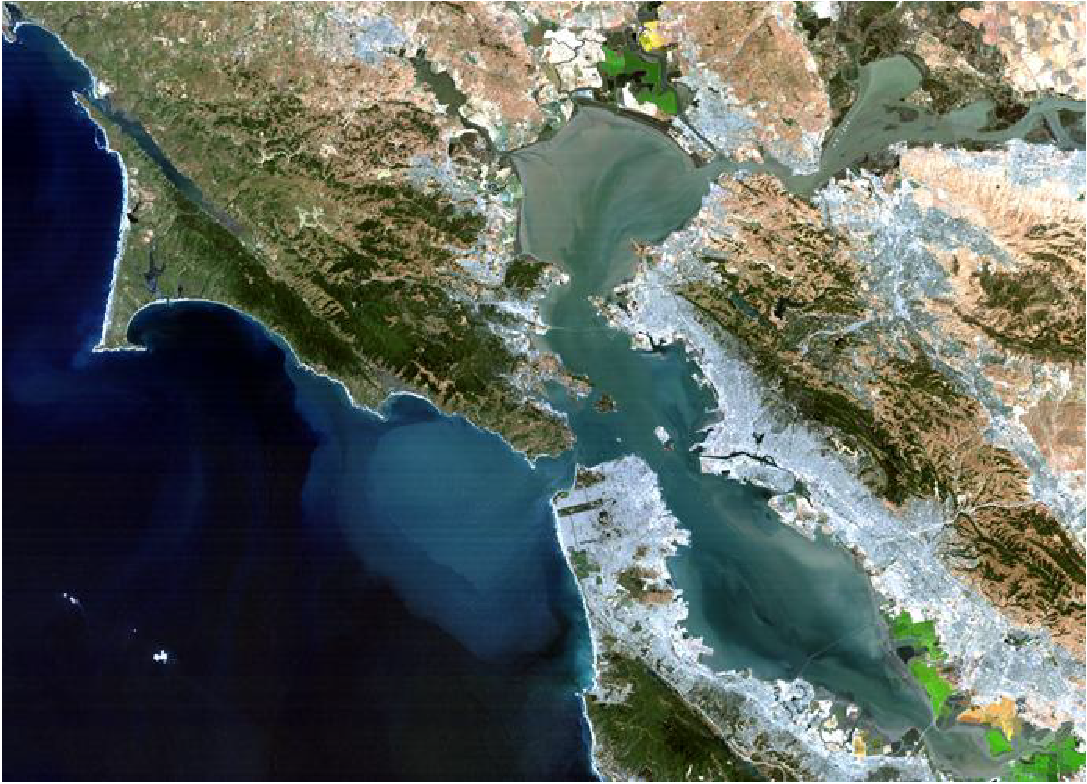
\includegraphics[scale=0.6]{image/plume2}
	\caption{Extent of sediment plume.}
	\label{fig:plume2}
\end{figure}

\begin{figure}
	\centering
		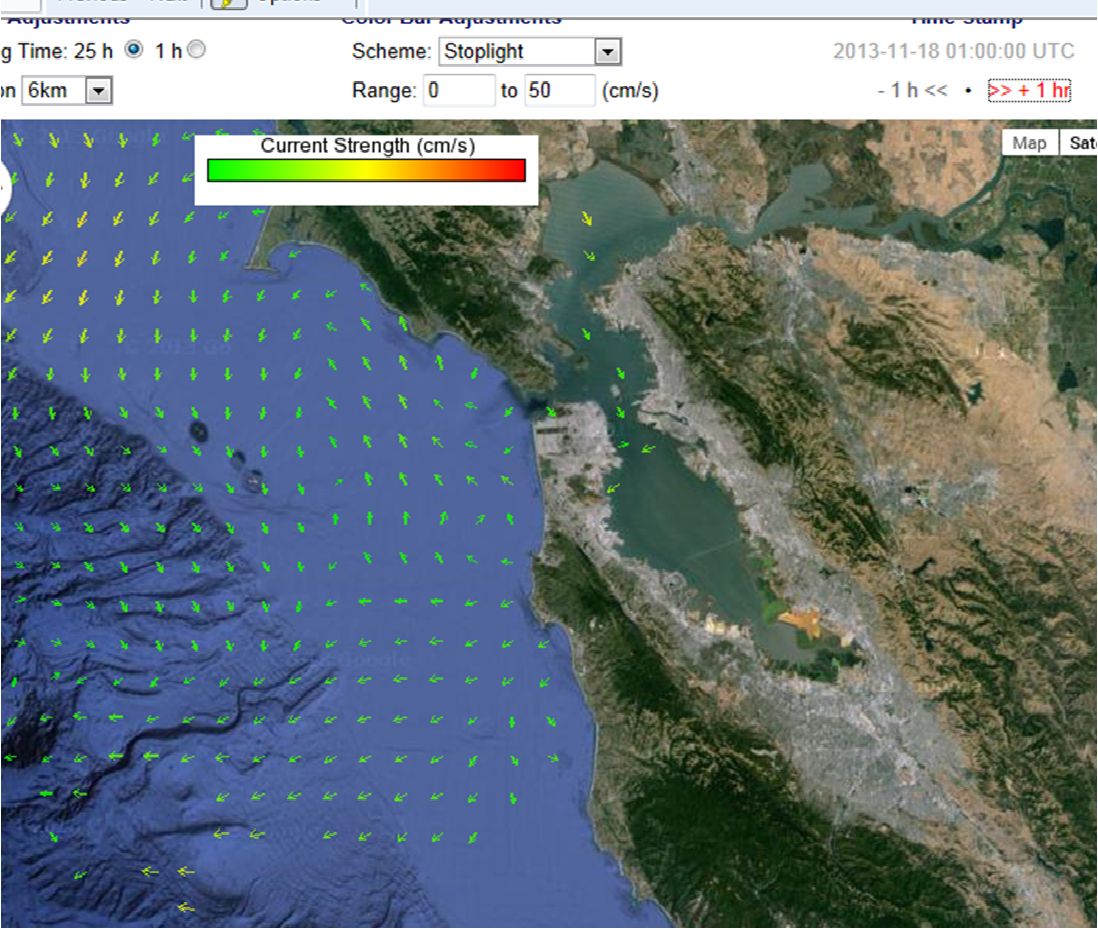
\includegraphics[scale=0.6]{image/hfradar.pdf}
	\caption{HF Radar surface currents (25 hour average, ****).}
	\label{fig:hfradar}
\end{figure}

\section{Flow Boundaries}
The main river inflows to the domain are shown in Figure ** and summarized in Table ***. As indicated, all our 
streamflows came from the USGS. Conductivity measurements were availble at some sites, others had to be approximated using
assumed constants or climatology as indicated in the table. The acquisition of the data involved some personal 
interaction and special requests and the subsequent processing is not easily reproducible, so it is our intention 
to release the data package for the calibration period along with the model. We also borrowed heavily from DSM2 inputs,
which have prepared in our section through 2011 and uses a lot of the data sources albeit with a greater reliance on
daily averaged data and CDEC as a data source. Occasionally there are large discrepencies between CDEC and USGS direct
sources of data; it just so happens that the beginning of our calibration in 2009 was one of those periods for Freeport,
with discrepencies reaching thousands of cubic feet per second (Figure ***).

As indciated in table ***, some data were made available to us as daily averages.
We interpolated the data using a rational histospline (****), which provides a (mostly) conservative, 
positivity and shape and peak preserving and accurate intepolation down to smaller time steps. 
Besides being inaccurate compared to this spline when applied to daily or monthly averaged data, 
the 24-hour square-wave produced by interpreting averages as flat lines can lead to results that are
subsequently misinterpreted as a daily or 14-day (through "`aliasing"') phenomenon. A 24-hour stairstep can also potentially influence model 
results at tidal frequencies and can degrade model performance due to the introduction of "`mini-tsunamis"' at the boundary. 


\subsection{Sacramento River boundary and extension}

\subsubsection{Boundary placement}
The upstream Sacramento boundary of the model is indicated in Figure ***.  The Sacramento River extends ***km north of I Street in Sacramento. Major tributaries have been lumped into the Sacramento channel, a point we will address again in our anticipated Yolo extension. The primary considerations for placement of the boundary were:

\begin{itemize}
	\item Availability of flow and bathymetric data
	\item Increasing complexity of the channel system (Yolo, Feather, American) north of I Street
	\item Need for the boundary to be free of tidal influence and boundary reflection
	\item Future extensions to Yolo requiring a boundary upstream of Fremont Weir.
	\item Performance and best practices with SELFE on upstream reaches
\end{itemize}

Of these criteria, the most constraining is the one concerning tidal influence and boundary reflection. Boundary reflection occurs when ocean tidal signals propagate all the way to the upstream boundary, conflict with incoming information and causes a reflected wave that moves back downstream and distorts conditions in the interior of the model. The effect of reflection on accuracy is significant and surprisingly far reaching. Figure *** shows the difference between model results at *** between a model truncated at I Street and a model extended beyond the zone of tidal influence near Knights Landing ****. Both models were forced by flows that were tidally filtered (ie, non-tidal in nature), which conflicts with conditions at I Street (see Figure ***) but not the upstream boundary. Clearly the effect of boundary reflection is felt as far as ***. For reference Figure *** compares water levels at I Street and the next available upstream gage at Fremont Weir demonstrating that the tidal signal is extinguished somewhere between these two sites.
 
\subsubsection{Boundary Data}

The simplification of flows into a single "`pseudo-Sacramento"' simplifies the system but requires a lumped estimate of flows into the Delta. In the Delta, the most upstream source of this combined flow is the USGS station at Freeport. We use data provided directly by the USGS because of large discrepencies between the USGS agency data and CDEC during the early months of our 2009 calibration period.  We also tidally filter the Freeport data, which has a significant tidal component that would be inappropriate if the data is lifted to the location of our boundary near Knights Landing. 

We use only flow and salinity to drive the model at the upstream Sacramento boundary. Overspecification using both flow and stage has been used successfully in Columbia River applications on steep river slopes, and is thought to help fix the upstream water levels at an appropriate elevation. Our only experiment with overspecification was at I Street where we found it was ****however we found that unless the flow and stage data are taken from 

\subsection{San Joaquin River}
The San Joaquin River Boundary is at Vernalis (Figure ***). As the contours in the figure show ***, south of Old River the San Joaquin transitions quickly from flat estuarine conditions to riverine. Field data indicates that Vernalis is naturally out of the zone of tidal influence. This is the the most important location in the Delta part of the model domain where flows are reported on the basis of stage observations and a rating curve. 

Unlike the field data, our model shows a small amount of tidal influence at the Vernalis boundary, indicating the model is a little underdamped in this part of the system. Some boundary reflection no doubt also results.

\subsection{Exports}
Export locations are indicated in Table ***. Our calibration period does not overlap with the CCC intake at **** . Data for the exports came from the original agencies or Dayflow, and the original data preparation comes from DSM2.

\subsubsection{Clifton Court and State Water Project}


\subsubsection{Contra Costa Water District}
The SELFE model was prepared to model three diversions at 


\subsection{CVP Tracy Pumping Plant}


\section{Delta agricultural sources and sinks}
The Delta islands are mostly agricultural, and diversions and returns of water from the islands significantly impact 
flow and water quality in the channels. The magnitude of the water quality impact varies with the seasons, as 
the balance between diversion, drainage and seepage changes. During summer months (including 2009), it is not
uncommon for the net sink of water due to consumptive use to exceed all of \gls{ndo}. This means that consumptive
use is not only a major driver of local water quality, but also a dominant contributor to the flow balance preventing
salinity intrusion from the ocean. 

Historical flow and water quality data has not traditionally been available for the islands. 
There have been recent efforts to map diversion pumps and return structures and it appears that many farmers in the Delta appear to log their diversions and returns now, but to the best of our knowledge these 
improvements have not yet been consolidated into a modeling product.  

\begin{figure}
	\centering
		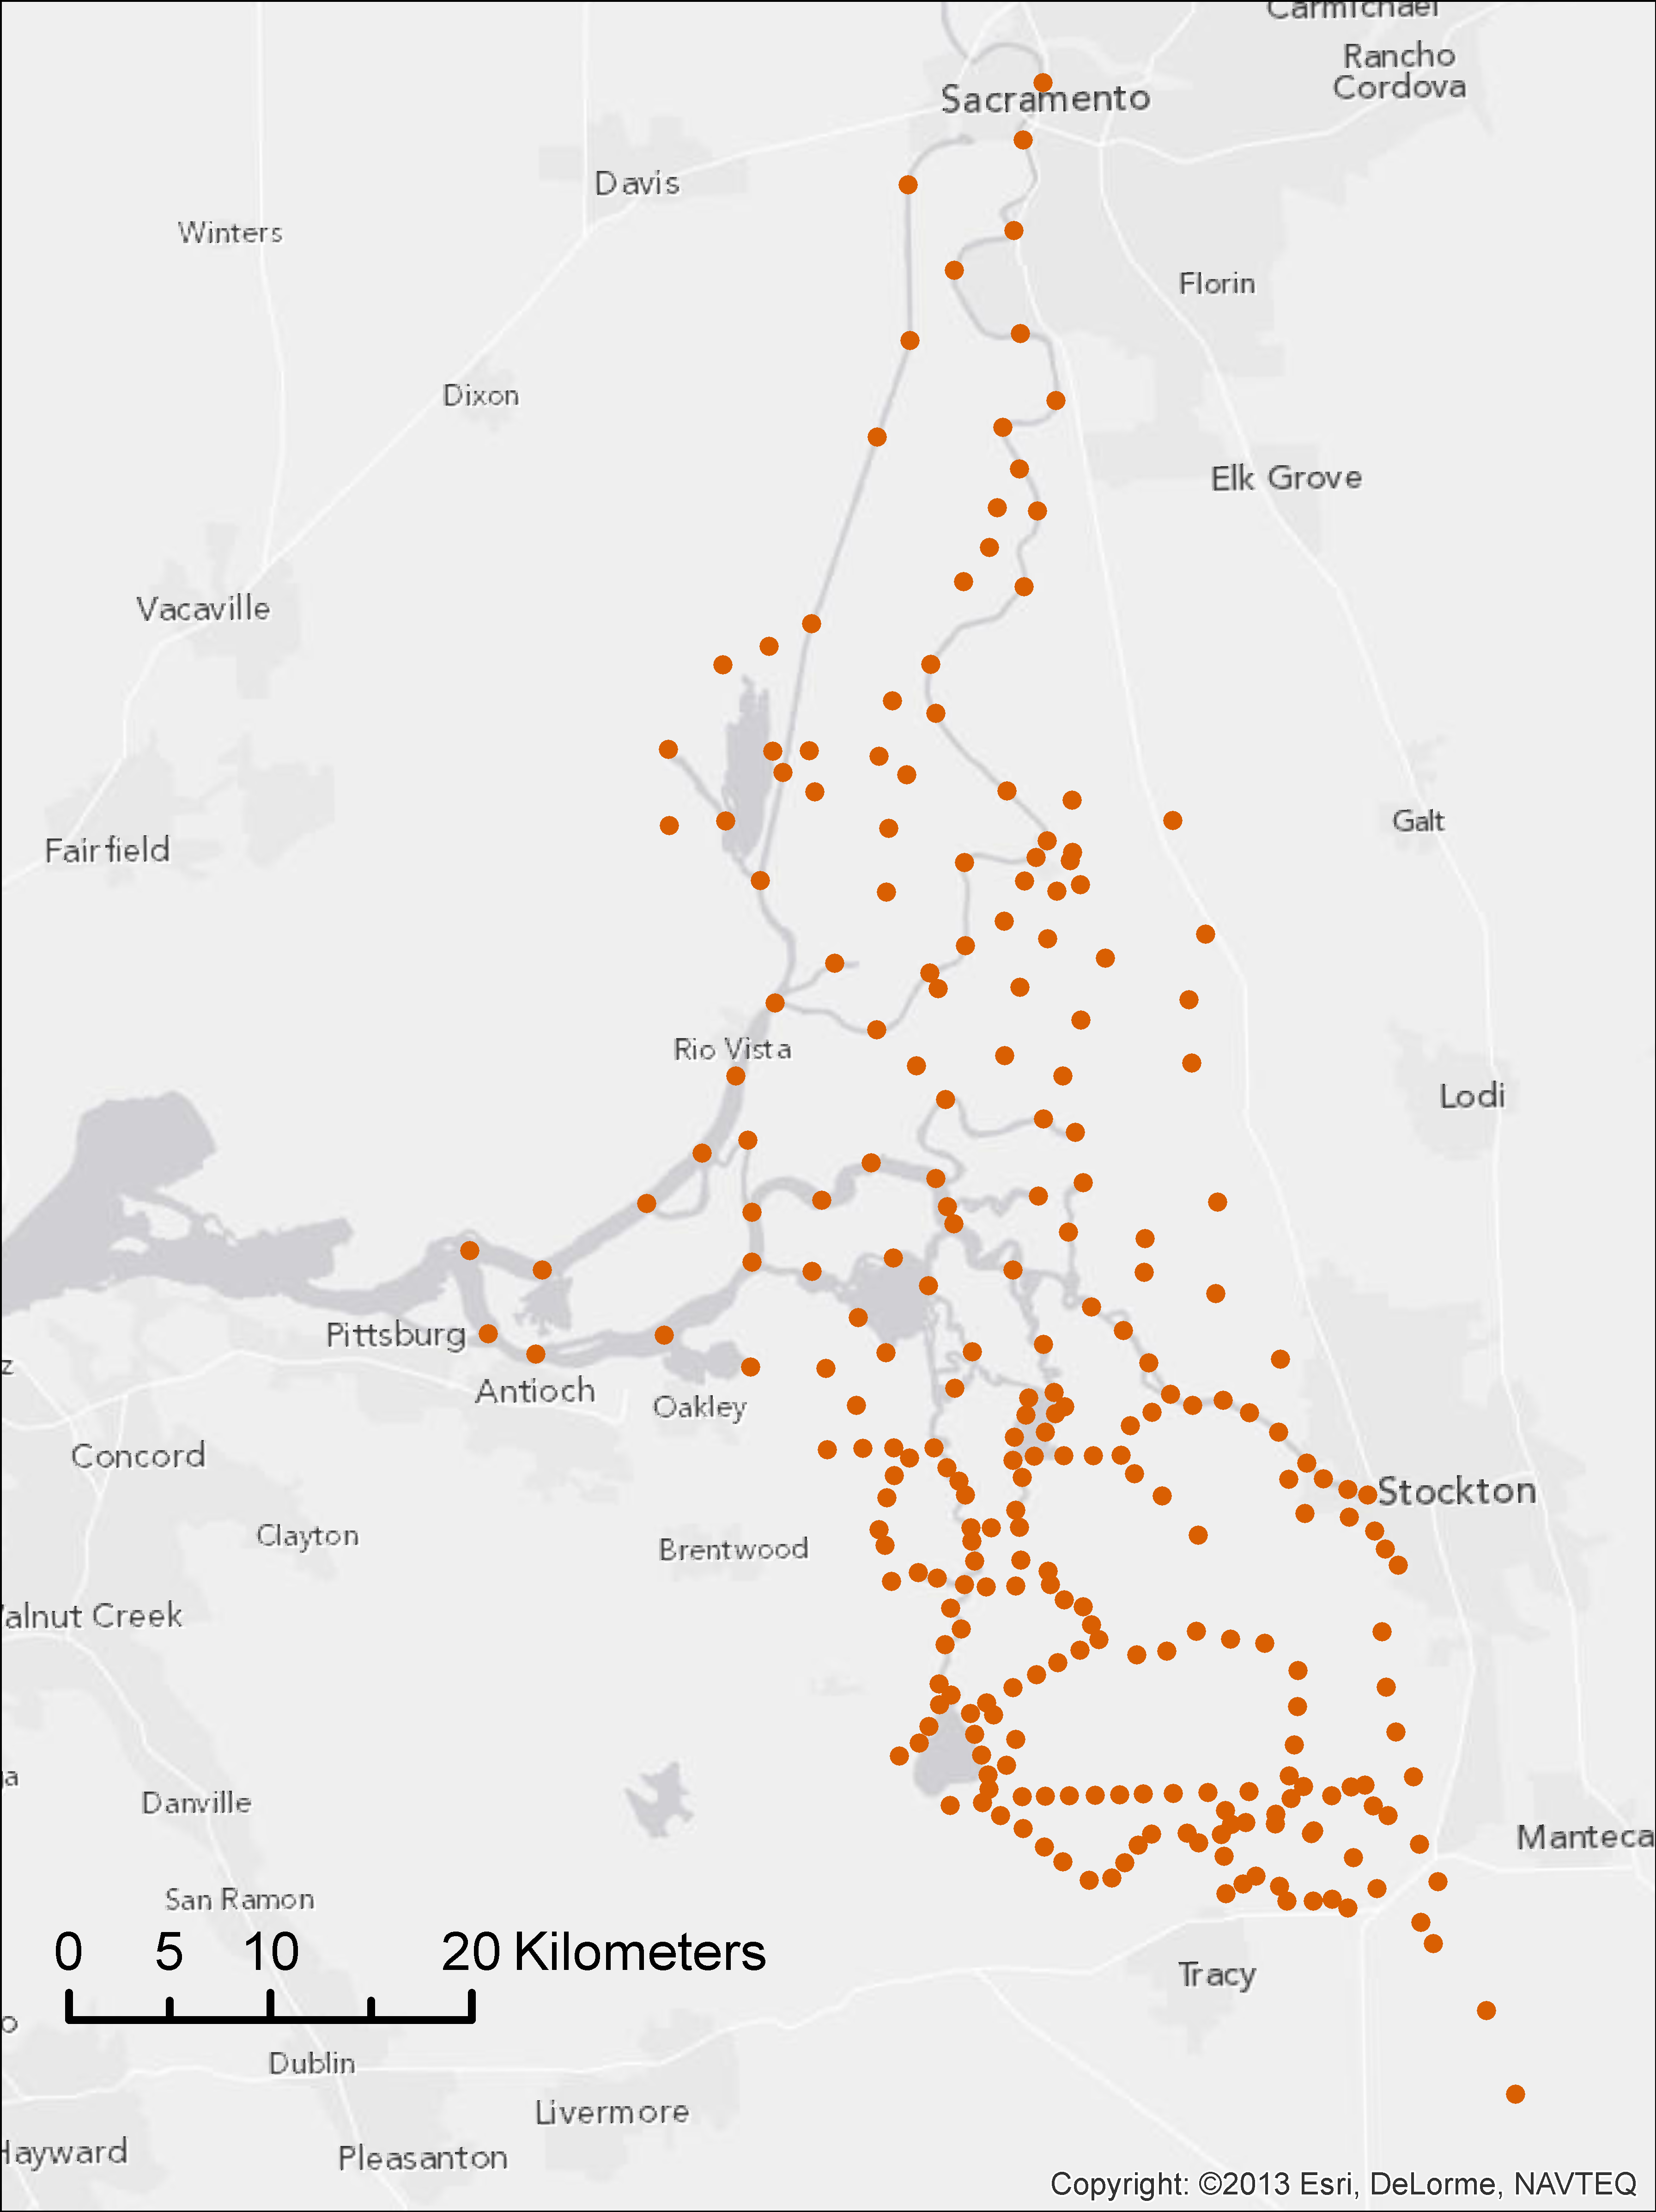
\includegraphics[scale=0.75]{image/dicu}
	\caption{Delta Island Consumptive Use diversion and return locations.}
	\label{fig:dicu}
\end{figure}

In the absence of field data, we use estimates from the DWR Delta Island Consumptive Use model
 (Mahadavan 1995, Jung 2000). The DICU model is centered on the islands (or regions), and performs 
a water balance that assumes land use and crop types and seeks to explain the resulting demand for water
in terms of precipitation, soil water balance, seepage and applied water.
The inferred fluxes to and from the Delta channels are then assigned to discrete locations in a second
step that is distinct from the water budget model. Although the assignment of locations 
is based on survey locations, the original locations are aggregated and the final locations of 
the sources are influenced by the location of nodes in \gls{dsm2}. The sites are shown in Figure \ref{fig:dicu}.

Delta consumptive use estimates can play an important part in model accuracy. 
During the summer months, agricultural water use can equal or exceed total
Net Delta Outflow in magnitude (Figure \ref{fig:ndo_vs_dicu}). Since outflow is a 
key quantity controlling salinity intrusion and consumptive use is the most uncertain
 components of outflow, DICU can play a controlling role in the accuracy of the model for salt.
In the one dimensional model DSM2, this error has been associated 
with overestimation of salinity in dry years including 2009. 

Because it is a monthly model, DICU also has difficulties representing event-scale runoff. 
DICU calculates runoff drainage based on excess precipitation (precipitation minus demand) 
and assumes that runoff is zero if there is no excess. The determination is made using monthly totals, 
which dilute short rainfall events over the full month and reduces the chances that they will be 
correctly identified as runoff. At best, the events are smeared in time; at worst, this 
miscategorization can trigger some accounting quirks with demand and cause volumes to be dropped altogether.

There is an event in mid-October of 2009 that illustrates how important isolated runoff events can be. This event
is shown in Figure \ref{fig:dayflow_oct_2009}, which plots Dayflow estimates of inflows, exports, precipitation and outflow for the latter part of 2009. The event in question begins on October 12, after which river inflows and exports go up modestly.
Because inflows and exports rise and fall roughly in tandem, their contributions to change in outflow tend to cancel out. 
Nevertheless, the Net Delta Outflow still goes up sharply because it is dominated by precipitation.
 
To examine the effect of runoff results, we simulated this period twice with identical parameters --  
once with DICU as-is and once substituting values from another consumptive use model \acrshort{detaw} during the storm period.
 \acrlong{detaw} is a daily water balance model for consumptive use that is still in development at DWR; it
is beyond the scope of this document to describe DETAW in detail, but we believe is more realistic for this type of event. 
Figure \ref{fig:detaw_vs_dicu} shows the difference between the two models in terms of agricultural drainage, which 
is the term that includes runoff. DICU ignores most of the volume of the storm and the rest is distributed over all of October.
DETAW, on the other hand, assumes that most of the precipitation that falls over the Delta contributes to drainage.

Figure *** shows the resulting model salinity results at several stations in the Bay and Delta. The simulation
based on DICU inputs do well until the storm, but after the event salinity remains high on as if nothing had happened. In 
contrast, salinity is driven down system-wide both in the DETAW driven model and in the field data. A difference of
3-4 psu (perhaps 4000***) develops immediately after the event in the west Delta and Bay stations and lasts for 2-3 months. 
Since the west corridor is the gateway to the Delta, the anomaly eventually reaches every Delta station. In contrast to 
any summer seasonal inaccuries in Net Delta Outflow, we found this issue to be very easy to identify with confidence, and we
retained the higher drainage for October and December for our calibration.

Up to now, we have described uncertainty due to consumptive use through the mechanism of salinity intrusion.
In addition, there is considerable uncertainty concerning the salinity of agricultural returns in early storms. 
Large spikes in of salt and other constituents occur following {\em first flush} precipitation 
events after dry periods. These spikes are evident in the historical records at mid and South Delta monitoring stations, and the sources and quantities involved have not been well characterized.

\begin{figure}
	\centering
		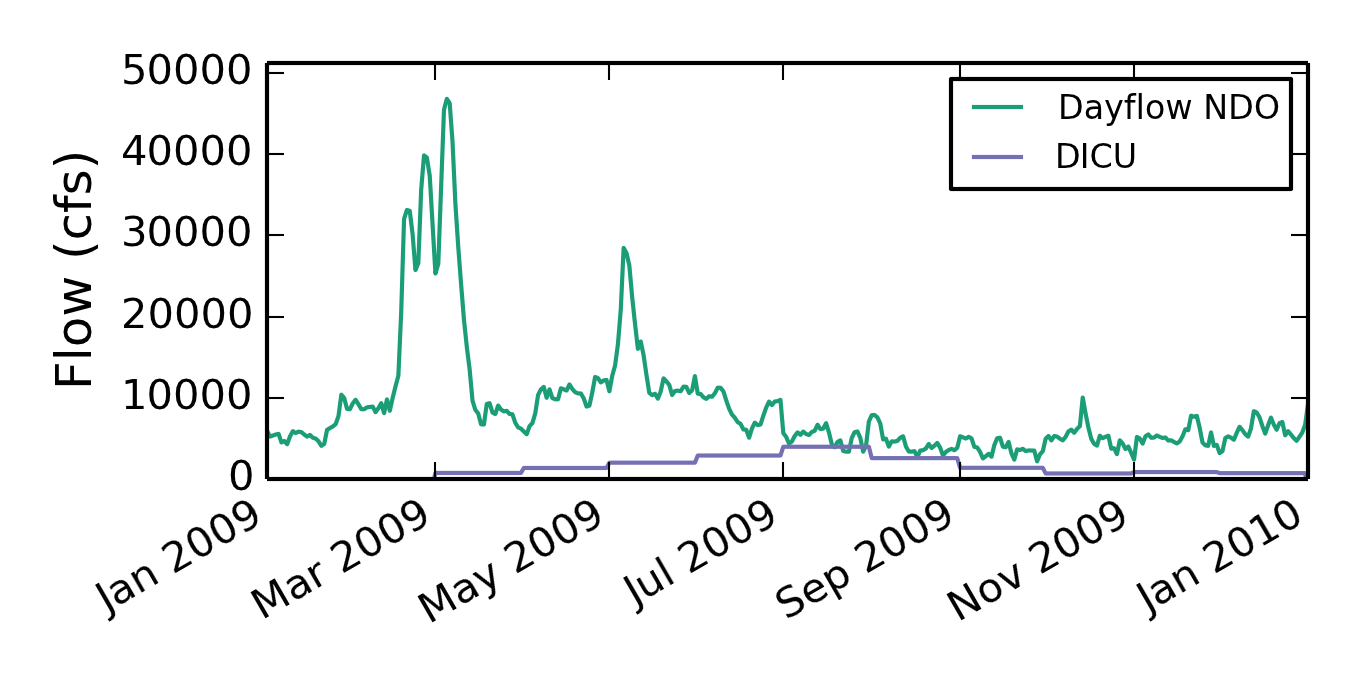
\includegraphics{image/ndo_vs_dicu}
	\caption{Net Delta Outflow and Delta Island Consumptive Use estimates for 2009.}
	\label{fig:ndo_vs_dicu}
\end{figure}

\begin{figure}
	\centering
		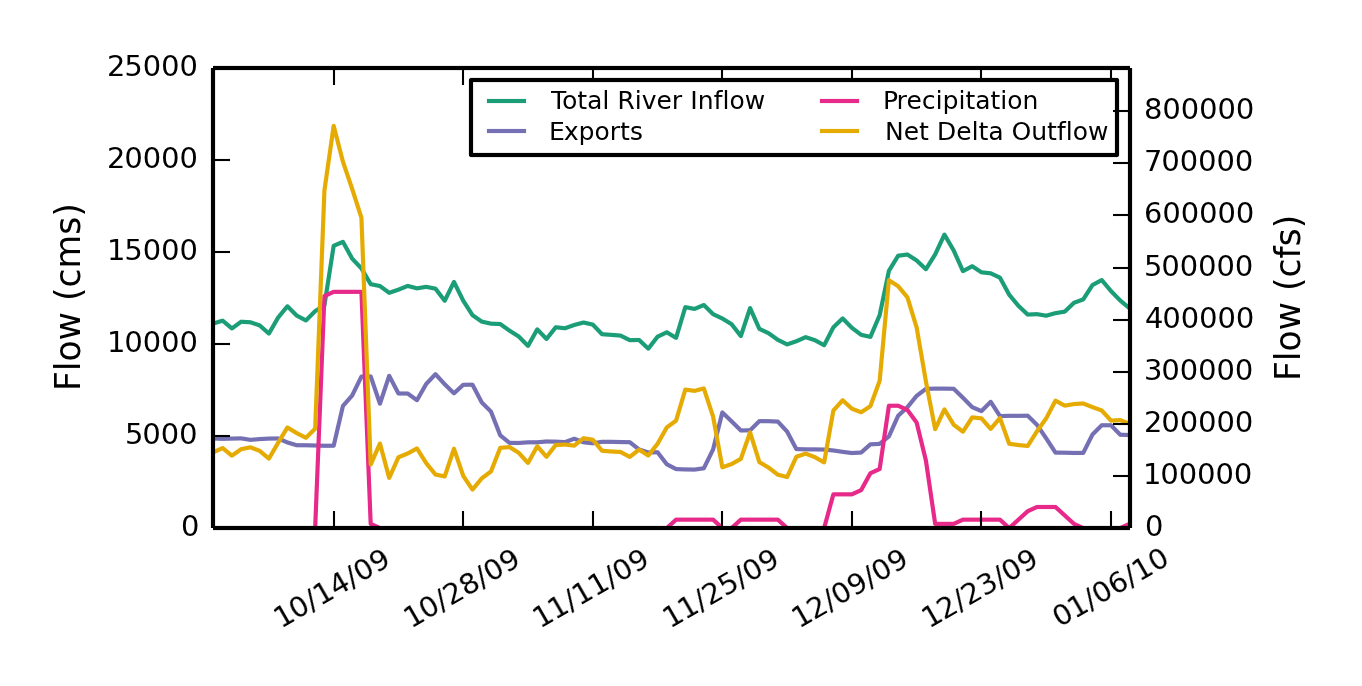
\includegraphics{image/dayflow_oct_2009}
	\caption{Dayflow estimates of inflows, exports, precipitation and Net Delta Outflow for the last part of 2009,
	including the storm period in mid-October.}
	\label{fig:dayflow_oct_2009}
\end{figure}

\begin{figure}
	\centering
		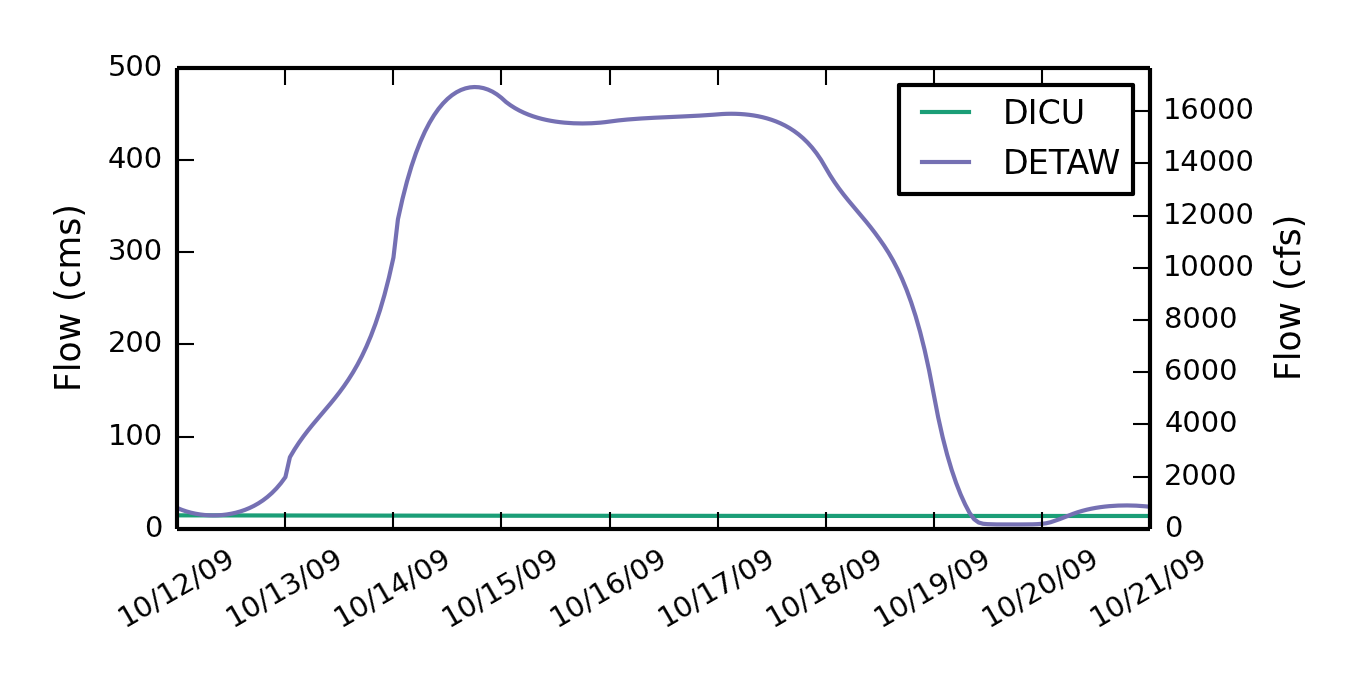
\includegraphics{image/detaw_vs_dicu}
	\caption{Estimates of agricultural drainage from DICU and DETAW around the period of the storm.}
	\label{fig:detaw_vs_dicu}
\end{figure}


\section{Atmospheric inputs}
When modeling flow and salinity transport, SELFE accepts spatiotemporal atmospheric 
input representing surface wind, atmospheric pressure
and precipitation over the domain. The most significant of these is thought 
to be wind, which alters flow patterns and induces mixing
resulting in as much as a 2 psu difference in salinity at Martinez. There is no unified approach to
modeling wind in the Bay-Delta region. Past work in the domain has either justified neglecting 
wind due to a short period of study \citep{Chua2011}
or used atmospheric inputs from a small set of representative 
stations situated on the water \citep{MacWilliams08,MacWilliams09}.

The approach we adopted is to use climate or weather reanalysis products that 
combine both a physical model and data assimilation. 
Numerous reanalysis products are available for the region at both climate 
(coarser) and weather (finer) scales. For our calibration we used winds
at 10m above ground from the \gls{narr} 
dataset from NOAA. This dataset is 32km in resolution, which is roughly 
the spacing of field stations used in \citep{MacWilliams08,MacWilliams09} and not fine enough
to resolve the width of the Bay or local spatial patterns of wind at 
the Golden Gate, South Bay, San Pablo Bay and Carquinez.

Through our collaborators in the SESAME project, we have access
to two much finer resolution wind fields 
from reanalysis products. The first is a 3km COAMPS model from the \gls{cencoos}. 
The second is a 1km WRF simulation from NASA unique 
to the SESAME project. The results of our collaborators indicate that the 3km model is able 
to reproduce many of the spatial features of the winds on the Bay, but
tends to reduce magnitudes, a common issue and certainly one that the NARR dataset suffers
from as well. The 1km model has higher peaks, but it was unclear to our collaborators 
that sensitivity for modeling justified the expense (months of supercomputer use) spent generating the 1km
product. 

The importance of atmospheric forcing must be balanced against the uncertainty and noise surrounding wind, 
the unknown (and relatively unknowable) effects of gusts and the expense of improving the wind and pressure data. 
Our principle goal in this project is to establish a robust model that can be used to examine hypothetical 
planning questions or future conditions. The calibration results presented 
in this document for the Bay suggest this is possible for scenarios that 
do not involve changed atmospheric conditions; to quantify our confidence for climate change scenarios 
involving big changes in the frequency of barometric events, further sensitivity analyses are required.


\section{Delta hydraulic control structures}
\label{sec-delta-structs}
Radial gates, barriers, culverts and other hydraulic structures are used in the the 
Delta and Suisun Marsh to help manage water quality, protect fish migration, maintain 
agricultural water supply (head) in the South Delta and control storage at Clifton Court. As part of this project
we added the ability to model a variety of such structures to SELFE. The implementation, 
which borrows concepts from DSM2 and HEC-RAS, uses fundamentally
1D parameterizations to allow the embedding of the structures in 
an otherwise medium resolution multi-dimensional mesh. More details are described in 
Section \ref{sec-structures}. 

Many structures in the Delta are seasonally installed or operated. Figures \ref{fig:gate_schedule_2009}
and \ref{fig:gate_schedule_2010} shows the operational schedule for 2009. 
Additional detail on what these operations mean is given 
in the individual control structure descriptions.


\begin{figure}
	\centering
		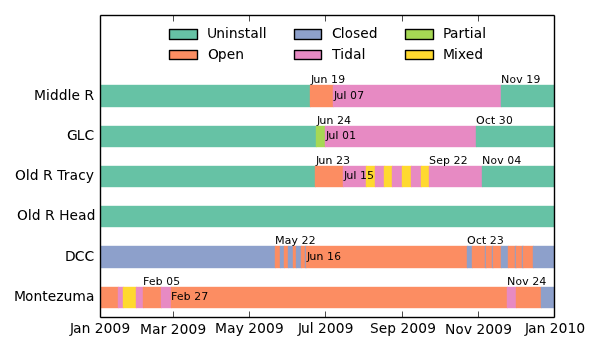
\includegraphics[width=\textwidth]{image/gate_schedule_2009}
	\caption{Delta hydraulic structure operations for 2009.}
	\label{fig:gate_schedule_2009}
\end{figure}

\begin{figure}
	\centering
		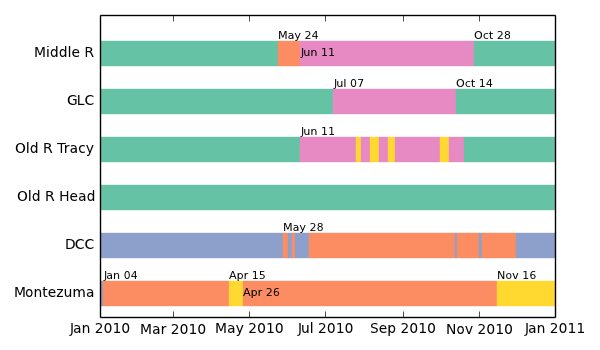
\includegraphics{image/gate_schedule_2010}
	\caption{Delta hydraulic structure operations for 2010.}
	\label{fig:gate_schedule_2010}
\end{figure}


\subsection{Delta Cross Channel} The \gls{dcc} is a permanent structure on the 
Sacramento River that comprises two 36.6m (120 ft) wide radial gates. The gate, along with the 
6,000ft cross channel connecting the  was completed by the \gls{usbr} in 1950-1951. The gate is 
opened in order to freshen water in the central Delta as well as for recreational boating use. 
The \gls{dcc} is operated seasonally with mandated closures to protect fisheries 
under \gls{d1641} and operational closures during periods of high flow to prevent scour. 

The openings and closings for our period of interest are given in 
Figures \ref{fig:gate_schedule_2009}-\ref{fig:gate_schedule_2009} and
 and are taken from the USBR historical log. In recent years, including the calibration period, the gate has 
remained closed for fish protection until Memorial Day weekend. In 2009, the cross-channel was 
open from June-October, although it was toggled open and closed frequently at the beginning and end of
that season. 

During the calibration period, the \gls{dcc} was operated with both gates either fully open or closed. 
This is the most common mode of use, although in the months before our calibration experiments 
were conducted with the gates operated frequently and sometimes in a partially open state. 

We model the cross channel as a radial gate. Flows through the channel 
seem to match observations well. We are not aware of any official gate rating for the cross-channel, 
although in a presentation before the \gls{cwemf} in 2006, K.T. Shum of EBMUD 
described problems in the fit of radial gate equations and advocated the use of 
flow contraction equations instead, such as those given by \citet{Matthias67}.
We have so far not been able to reproduce the difficulties leading to these comments.

\subsection{Clifton Court Forebay Gates} Five radial gates control flow into the Clifton Court Forebay. The gates are each *** wide (**m), with a sill elevation of *** m NAVD (**** ft NAVD ,or *** ft NGVD). Each of the five gates can be independently operated although they are most commonly operated in tandem. 

The gates are operated in accordance with an agreement with the South Delta Water Agency to maintain water levels in the surrounding region. The resulting {\em Priority System} describes when in the tide cycle the gates may be opened. The priorities schedule is shown in Figure ***. The most common priority is {\em Priority 3}, which under normal tidal circumstances allows the gates to open 1 hour after the lower low tide, close 2 hours after the higher low tide, open again 1 hour before the higher high tide, and close 2 hours before the next lower low tide. This schedule specifies the maximum periods when gates may be opened to inflow; the gates can be closed early if daily inflow quotas have been met and the gates are always closed to outflow.

\begin{figure}
	\centering
		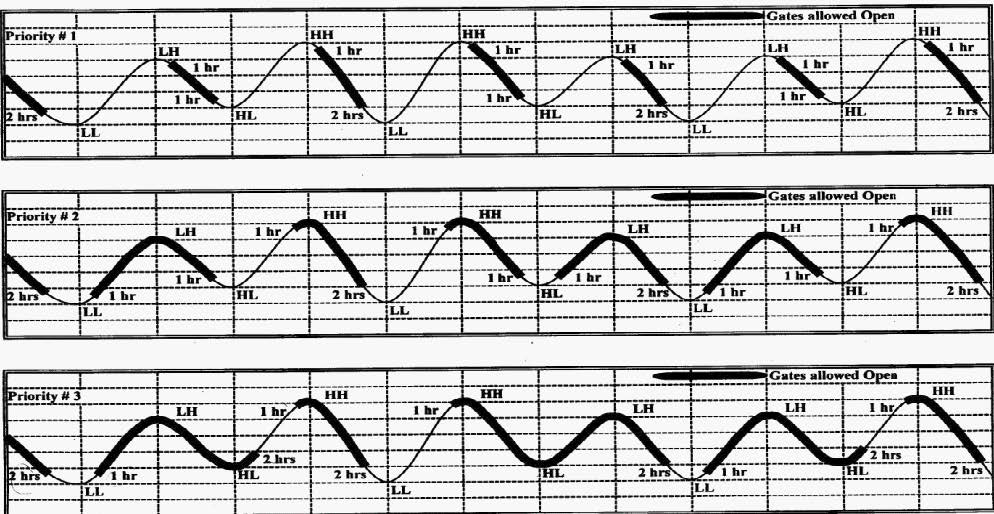
\includegraphics{image/ccfb_priority}
	\caption{Clifton Court Gate Priority Schedule.}
	\label{fig:ccfb_priority}
\end{figure}

Unlike other radial gates in the system, the CCFB gates are often operated such that the upstream side of the gate is submerged and the downstream side is submerged or (possibly) partially submerged. The term {\em partially submerged} is based on the state on the interior side and refers to the transition between {\em free flow} and {\em submerged flow} cases as indicated in Figure \ref{fig:radial_gate}. Partial submergence is something of a grey area in the literature on radial gates -- it is a regime that is difficult to characterize or even identify. Traditional measures of partial submergence, such as those implemented by the Army Corps of Engineers HECRAS, are based on the ratio of tailwater to headwater ($0.6 < y_3/y_1 < 0.8$). This ratio almost always exceeds 0.8 at Clifton Court, so by this criterion the gate is always fully submerged. More recent work on radial gates \citep{Clemmens03,Wahl05} interprets submergence based on whether downstream flow depth is greater than the theoretical free-jet thickness for a given gate opening. This leads to a more greater likelihood of characterization of partial submergence.

Operations near the partial submergence threshold make it challenging to develop a flow rating that applies well over the full range of gate heights and water levels. The DWR \gls{dfd} has a set of equations developed by \cite{Hills1988} that have been cited extensively, but these equations were developed over a very limited range of gate heights and are thought to be in error by as much as 40\% under some conditions. The DWR Delta Field Division calculates these values at ten minute intervals, but we are not aware of any circumstances at the DWR where the resulting flows are used without significant reinterpretation. The Delta Modeling Section is been developing a new rating for the gate for some time, but the collection of data for certain flow and stage combinations has been delayed by operational changes and a mechanical failure at one of the gates. DSM2 uses an orifice equation calibrated heuristically based on storage changes in Clifton Court; we believe this is a justifiable single-equation approach, but have not yet had an opportunity to verify how well it reproduces fluxes into Clifton Court.

For historical calibration (as opposed to hypothetical scenarios), the issue of improving the gate rating can be deferred because other supporting data are available. \citet{MacWilliams13} suggest a methodology whereby the ten minute Hills equation gate flows are scaled on a daily basis to match the historical daily flux into Clifton Court estimated by Dayflow. The Dayflow estimate is based on a mass balance on the reservoir that includes daily fluctuations in CCFB water levels, \gls{swp} and \gls{bbid}. We did not include an evaporation correction. The resulting flows reproduce the daily volume in CCFB by definition, and can be prescribed directly in SELFE using a {\em flow transfer} (see Section \ref{sec-transfer}). The main difficulty we encountered with this approach was that the flow balance between the gates and pumps is delicate and easily disrupted by things like interpolation techniques or FEM mass conservation errors -- a long term average bias of 1 cms will accumulate to a very appreciable drift in CCFB water levels.

\begin{figure}
	\centering
		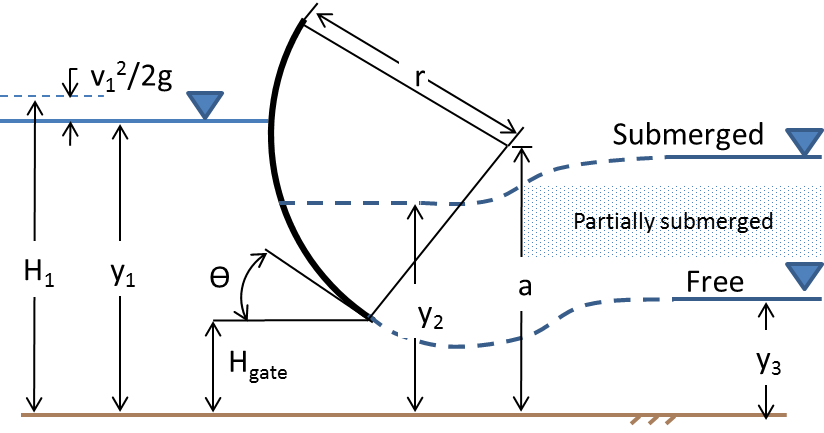
\includegraphics{image/radial_gate}
	\caption{Free and submerged downstream flow through a radial gate. The upstream is submerged}
	\label{fig:radial_gate}
\end{figure}


\subsection{Montezuma Slough Salinity Control Gates}
The Suisun Marsh Salinity Control Gates facility consists of three 11m (36ft) wide radial gates, a 36.6m (120ft) set of
flashboards and a 6.1m (20ft) wide boat lock. 

The gate is designed to operate tidally, restricting flow of higher salinity water 
from Grizzly Bay into Montezuma Slough on the incoming tides, and passing lower salinity 
Sacramento River water during ebb tides. Tidal operation of the gate lowers salinity 
in Suisun Marsh channels and results in a net movement of water from east to west. When the gates
 are left open and \gls{ndo} is low, the net movement is slightly west-to-east.

The salinity control structure radial gates can be operated operated tidally beginning in in early 
October and, depending on salinity conditions, may continue operating in this way 
through the end of the control season in May. As shown in Figure \ref{fig:gate_schedule_2009} and \ref{fig:gate_schedule_2010} 
the window of tidal operation in 2009-2010 was actually just a few months. 

The flashboards are wide stoplogs that can be removed to allow unimpeded flow when salinity conditions in the Marsh are favorable. The boat lock tends to be held open when the flashboards are in to allow improved fish passage and is closed when the flashboards are out. 

The Bay-Delta SELFE model includes all three subdevices at the control structure. 
The weir is modeled using a radial gate using the HEC formulation. Coefficients were taken from
the DSM2 inputs and were not adjusted. The boat lock is modeled as a weir, and the flashboards as a rectangular orifice. 
Dimensions and coefficients for these structures were also borrowed from 
DSM2 inputs. 

\begin{figure}
	\centering
		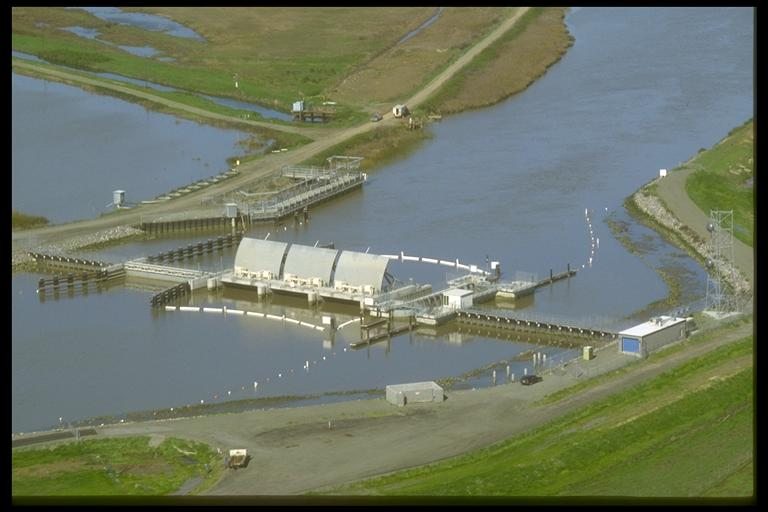
\includegraphics[scale=0.5]{image/smscg}
	\caption{Montezuma Salinity Control Gate.}
	\label{fig:montezuma}
\end{figure}

\subsection{South Delta Temporary Barriers} The South Delta Temporary Barriers have been installed in
various configurations in four locations in the South Delta since 1991. They include one fish barrier 
at the Head of Old River and three seasonal rock barrier sites on Middle River, Grantline Canal and Old River (Figure **). The fish barrier is intended to protect migrating San Joaquin River Chinook salmon from being entrained by 
water project pumps. The three agricultural barriers are intended to preserve water levels 
and improve water quality in the South Delta for agricultural water users along those channels. 

The agricultural barriers are all designed in roughly similar way, including a rock barrier 
with a crest above sea level as well as a set of 4ft diameter (1.22m) diameter 
culverts with optional flap gates for tidal operation.  The configuration of the culverts varies by
site: the Middle River has three at the north levee side and three at the south side, the GLC barrier 
has all six culverts on the south levee side, and the Old River barrier has all nine culverts situated in the middle
under the weir. At Middle River and the Grantline Canal barriers, the bank of culverts stay in year round.
In all cases, weir and pipe flow are summed as if they were independent, ignoring the complications 
arising from interaction. Porosity of the rock barriers themselves is also ignored.

To the best of our knowledge, the flow coefficients of the agricultural barriers 
have not been studied in isolation -- ie, by observing velocity directly upstream 
or downstream using \glspl{uvm} or \glspl{adcp}.
We began by using weir and culvert coefficients from DSM2, but found that these coefficients
were high in the context of SELFE (and indeed are high according to published recommendations). This
 seems particularly true in before the culverts were replaced in 2010-2011. As a result, we reduced both culvert and
weir coefficients to less than half their original values.

\section{Domain variations (Bay-only, Delta-only)}
Although the final 'production' simulations were carried out on the Bay-Delta grid, 
we also conducted some earlier experimental work with Bay-only grids, in order to sort some 
calibration issues in the lower estuary more efficiently. The grid (Figure ***) 
is much smaller than the Bay-Delta grid, with only ~23K nodes. This allows much 
quick turn-around time for experiments involving Bay dynamics. The model skills are 
largely comparable on the two grids, with slightly better results from the larger grid, 
partly due to the reduction of reflection at the river boundaries
and natural exchange through Threemile Slough. For the Bay-only
grid, the river boundaries are located at Jersey Point and Rio Vista, with measured stages, flows and EC imposed there. 
No "False Delta" was used as was the case in early work by most other authors.

Also of interest to the Department is a Delta-only domain with a boundary at Martinez -- possibly
with less vertical resolution or even in 2D. SELFE has often been used in this way and
we have developed scripts to perform the necessary kind of domain chopping, 
but our focus thus far has been on the full domain in 3D.

\section{Domain-specific sources of uncertainty}
The current state of the model encompasses many important facets of the Bay-Delta system, particularly the upper estuary and Delta where operational details can be most critical. Nevertheless, some details of the Delta remain unknown difficult to model
  \subsection{Delta consumptive use}

	
	\subsection{Bathymetry}
  The present project has advanced the 

	\subsection{Vegetation and friction}
	


